\documentclass{article}
\usepackage[margin=1in]{geometry}
\usepackage[nodisplayskipstretch]{setspace}
\usepackage{amsmath, nccmath, bm}
\usepackage{amssymb}
\usepackage{enumitem}
\usepackage{graphicx}
\usepackage{float}
\usepackage{listings}
\usepackage{hyperref}
\usepackage[svgnames]{xcolor}
\usepackage{indentfirst}
%\usepackage{chngcntr}
%\counterwithin{table}{section}
\graphicspath{
{./images}}

%\hypersetup{
%    colorlinks=true,
%    linkcolor=black,
%    filecolor=black,      
%    urlcolor=blue
%    }

\newcommand{\zerodisplayskip}{
	\setlength{\abovedisplayskip}{0pt}%
	\setlength{\belowdisplayskip}{0pt}%
	\setlength{\abovedisplayshortskip}{0pt}%
	\setlength{\belowdisplayshortskip}{0pt}%
	\setlength{\mathindent}{0pt}}
	
\definecolor{vgreen}{RGB}{104,180,104}
\definecolor{vblue}{RGB}{49,49,255}
\definecolor{vorange}{RGB}{255,143,102}

\lstdefinestyle{verilog-style}
{
    language=Verilog,
    basicstyle=\small\ttfamily,
    keywordstyle=\color{vblue},
    identifierstyle=\color{black},
    commentstyle=\color{vgreen},
    numbers=left,
    numberstyle=\tiny\color{black},
    numbersep=10pt,
    tabsize=8,
    moredelim=*[s][\colorIndex]{[}{]},
    literate=*{:}{:}1
}

\lstset{style={verilog-style},showstringspaces=false}

\lstdefinestyle{nocoloring}{
    keywordstyle=\color{black},
    commentstyle=\color{black},
    stringstyle=\color{black}
}

\makeatletter
\newcommand*\@lbracket{[}
\newcommand*\@rbracket{]}
\newcommand*\@colon{:}
\newcommand*\colorIndex{%
    \edef\@temp{\the\lst@token}%
    \ifx\@temp\@lbracket \color{black}%
    \else\ifx\@temp\@rbracket \color{black}%
    \else\ifx\@temp\@colon \color{black}%
    \else \color{vorange}%
    \fi\fi\fi
}
\makeatother

\newcommand{\code}[1]{%
	\colorbox{Gainsboro}{\texttt{#1}}%
}

\title{Lab 3}
\author{Owen Sowatzke}
\date{April 21, 2025}

\begin{document}

	% \offinterlineskip
	% \setlength{\lineskip}{12pt}
	% \zerodisplayskip
	\maketitle
	
	\section{Introduction}
	
	In this lab, we perform design and verification for an ARM 8-bit microprocessor. We start by simulating a SystemVerilog model of the microprocessor in NC verilog. Then, we design 8-bit AND and OR wordslices in Cadence Virtuoso. For each of these wordslices, we create a schematic, symbol, and layout. Then, we incorporate each of our wordslices into the ALU and update its schematic and layout. Similarly, we update the datapath layout with our updated ALU. At each stage of the design, we verify our layouts using DRC and LVS. Finally, we create a netlist from our design and validate its behavior in simulation. 
	
	\section{AND Wordslice}
	
	In this section, we perform design and verification of our AND wordslice. Our wordslice specifically contains 8 \texttt{and2\_1x} gates from the \texttt{muddlib11} library. The resulting schematic is shown in Figure \ref{fig::and2_1x_8_schematic}. Note the vectorized ports and component instances.
	
	\begin{figure}[H]
		\centerline{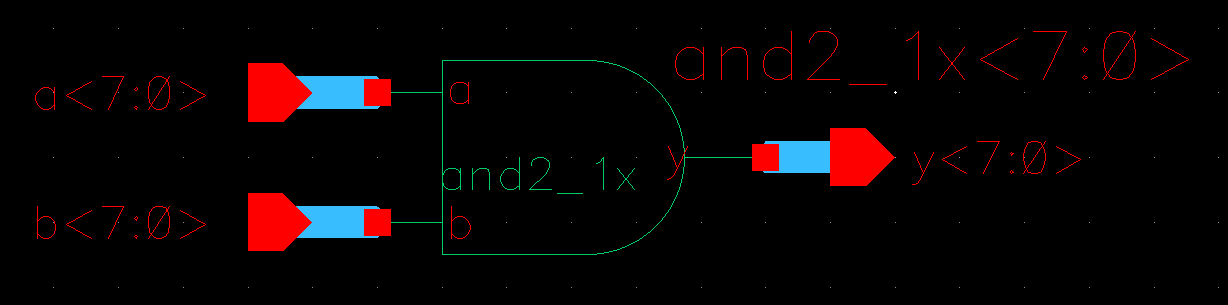
\includegraphics[width=0.5\textwidth]{and2_1x_8_schematic.png}}
		\caption{Schematic for AND Wordslice}
		\label{fig::and2_1x_8_schematic}
	\end{figure}
	
	\noindent Next, we create a symbol for our AND wordslice. For this step, we start with a copy of the \texttt{and2\_1x} symbol and make small incremental updates. Our wordslice symbol with these updates is shown in Figure \ref{fig::and2_1x_8_symbol}. Note that the port names and wire widths have been updated to reflect the vectorized inputs and outputs.
	
	\begin{figure}[H]
		\centerline{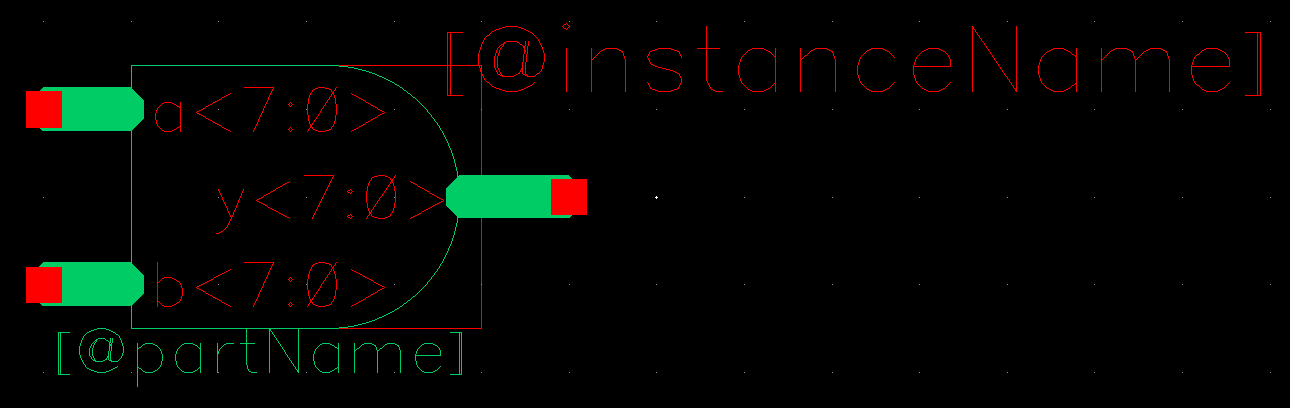
\includegraphics[width=0.5\textwidth]{and2_1x_8_symbol.png}}
		\caption{Symbol for AND Wordslice}
		\label{fig::and2_1x_8_symbol}
	\end{figure}
	
	\noindent Then, we create a layout for our wordslice. To create the layout, we start with a mosiac of AND gates. Then, we place input and output ports on each of our gates. However, in this configuration, virtuoso shorted each of the vectorized pins (or incorrectly reported them as shorted).
	
	  between each of our input and output ports.
	
	\section{NOR Wordslice}
\end{document}